\documentclass[11pt,a4paper]{article}

% ------------------------------------------------------------
% Packages
% ------------------------------------------------------------
\usepackage[margin=2.2cm]{geometry}
\usepackage[T1]{fontenc}
\usepackage{lmodern}
\usepackage{microtype}
\usepackage{graphicx}
\usepackage{booktabs}
\usepackage{array}
\usepackage{float}
\usepackage{caption}
\usepackage{subcaption}
\usepackage{xcolor}
\usepackage{enumitem}
\usepackage{listings}
\usepackage{fancyhdr}
\usepackage[hidelinks]{hyperref}

\captionsetup{font=small,labelfont=bf}
\setlist{itemsep=2pt,topsep=4pt}
\renewcommand{\arraystretch}{1.15}

% ------------------------------------------------------------
% Draft switch: set \drafttrue to show red TODO markers,
% \draftfalse to hide them for the final PDF.
% ------------------------------------------------------------
\newif\ifdraft
\drafttrue
\newcommand{\todo}[1]{\ifdraft\textcolor{red}{\textbf{[TODO: #1]}}\fi}

% ------------------------------------------------------------
% Team information (edit here)
% ------------------------------------------------------------
\newcommand{\TeamID}{T08}

\lstset{
  basicstyle=\ttfamily\footnotesize,
  breaklines=true,
  frame=single,
  backgroundcolor=\color{black!4},
  rulecolor=\color{black!25},
  columns=fullflexible,
  keepspaces=true
}

\pagestyle{fancy}
\fancyhf{}
\lhead{\small AI Platforms -- Assignment 1}
\rhead{\small Team \TeamID}
\cfoot{\small\thepage}
\renewcommand{\headrulewidth}{0.3pt}

\begin{document}

% ------------------------------------------------------------
% Title block
% ------------------------------------------------------------
\begin{center}
  {\large Faculty of Computers and Data Science, Alexandria University}\\[2pt]
  {\large AI Platforms -- Fall 2026}\\[2pt]
  Professor: Dr.\ Yasser Foad \quad|\quad TA: Ahmed Yousri\\[14pt]
  {\LARGE\bfseries Assignment 1: Medical Image Classification}\\[4pt]
  {\Large Brain Tumor MRI -- TensorFlow vs.\ PyTorch, Served with FastAPI}\\[12pt]
  {\large\bfseries Team ID: \TeamID}\\[4pt]
  Team members: {Rokayya Aly, Mohamed ElBassat}
\end{center}
\vspace{4pt}
\hrule
\vspace{8pt}

% ------------------------------------------------------------
\section*{Summary}
We classified brain MRI slices into four classes (glioma, meningioma, notumor, pituitary) using transfer learning with two ImageNet-pretrained architectures, ResNet-50 and EfficientNet-B0, each implemented in both PyTorch and TensorFlow/Keras (four models in total). Grad-CAM was applied in both frameworks. The best model, \textbf{PyTorch ResNet-50 (test accuracy 84.06\%)}, is served through FastAPI.

\begin{table}[H]
\centering
\caption{Test-set results for all four models (1{,}600 images; precision, recall and F1 are weighted averages over the four classes).}
\label{tab:summary}
\begin{tabular}{llcccc}
\toprule
Framework & Architecture & Accuracy & Precision & Recall & F1 \\
\midrule
PyTorch    & ResNet-50 \textbf{(deployed)} & \textbf{0.8406} & \textbf{0.8485} & \textbf{0.8406} & \textbf{0.8368} \\
PyTorch    & EfficientNet-B0               & 0.8369 & 0.8458 & 0.8369 & 0.8320 \\
TensorFlow & ResNet-50                     & 0.6081 & 0.6156 & 0.6081 & 0.6019 \\
TensorFlow & EfficientNet-B0               & 0.2594 & 0.2963 & 0.2594 & 0.1541 \\
\bottomrule
\end{tabular}
\end{table}

% ------------------------------------------------------------
\section{Dataset and Train / Validation / Test Split}
All teams use the Brain Tumor MRI Dataset (Kaggle, \texttt{masoudnickparvar/brain-tumor-mri-dataset}). Images are 2D MRI slices labelled \texttt{glioma}, \texttt{meningioma}, \texttt{notumor} or \texttt{pituitary}. The dataset ships with a \texttt{Training} and a \texttt{Testing} folder. We kept the official \texttt{Testing} folder untouched as our test set and carved the validation set out of \texttt{Training} (15\%, random, seed 42).

\begin{table}[H]
\centering
\caption{Dataset split (identical sizes in both frameworks).}
\label{tab:split}
\begin{tabular}{lrl}
\toprule
Split & Images & Source \\
\midrule
Train      & 4{,}760 & 85\% of the \texttt{Training} folder \\
Validation &   840   & 15\% of the \texttt{Training} folder (seed 42) \\
Test       & 1{,}600 & official \texttt{Testing} folder (400 per class) \\
\midrule
Total      & 7{,}200 & \\
\bottomrule
\end{tabular}
\end{table}

\noindent The class order is alphabetical in both frameworks (\texttt{glioma}, \texttt{meningioma}, \texttt{notumor}, \texttt{pituitary}), which matches the order required by the API contract. Note that the validation subsets are drawn with each framework's own seeded splitter (\texttt{random\_split} in PyTorch, \texttt{validation\_split} in Keras), so they are the same size but not guaranteed to contain the same images; the test set is identical.

% ------------------------------------------------------------
\section{Preprocessing and Data Augmentation}\label{sec:preproc}
All images are resized to $224\times224$ RGB (the input size of both pretrained backbones). Augmentation is applied to the training set only and is deliberately mild: horizontal flips and small rotations are plausible variations in head pose and scanner orientation, whereas aggressive colour or contrast jitter could alter the intensity patterns that carry diagnostic information in MRI.

\begin{table}[H]
\centering
\caption{Preprocessing and augmentation in each framework.}
\label{tab:preproc}
\begin{tabular}{p{3.3cm}p{5.6cm}p{5.6cm}}
\toprule
 & \textbf{PyTorch} & \textbf{TensorFlow / Keras} \\
\midrule
Resize        & \texttt{Resize((224,224))} & \texttt{image\_size=(224,224)} \\
Scaling       & \texttt{ToTensor()} (pixels to $[0,1]$) & \texttt{Rescaling(1/255)} (pixels to $[0,1]$) \\
Normalisation & ImageNet mean/std \newline $(0.485,0.456,0.406)/(0.229,0.224,0.225)$ & none beyond $1/255$ \\
Augmentation (train only) & \texttt{RandomHorizontalFlip}, \texttt{RandomRotation(15)} (up to $\pm15^\circ$) & \texttt{RandomFlip("horizontal")}, \texttt{RandomRotation(0.1)} (up to $\pm10\%$ of a full turn, i.e.\ $\pm36^\circ$) \\
Validation / test & resize + normalise only & resize + rescale only \\
\bottomrule
\end{tabular}
\end{table}

\noindent The two pipelines are therefore \emph{not} identical: they differ in normalisation and in the rotation range. This matters for the framework comparison in Section~\ref{sec:fwcomp}.

% ------------------------------------------------------------
\section{PyTorch Models}
\subsection{Architecture and transfer-learning setup}
Both networks are loaded from \texttt{torchvision} with ImageNet weights. \textbf{All backbone parameters are frozen} (\texttt{requires\_grad=False}) and only the final classification layer is replaced by a new randomly initialised \texttt{Linear} layer with 4 outputs and trained. This is feature-extraction style transfer learning, not full fine-tuning of the backbone.

\begin{itemize}
  \item \textbf{ResNet-50:} \texttt{fc}: $2048\to4$ ($8{,}196$ trainable parameters; $\approx23.5$M frozen backbone parameters). Grad-CAM layer: \texttt{layer4[-1]}.
  \item \textbf{EfficientNet-B0:} \texttt{classifier[1]}: $1280\to4$ ($5{,}124$ trainable parameters; $\approx4.0$M frozen backbone parameters), keeping torchvision's dropout layer. Grad-CAM layer: \texttt{features[-1]}.
\end{itemize}

\subsection{Hyperparameters}
\begin{table}[H]
\centering
\caption{Hyperparameters (identical for both architectures and both frameworks unless noted).}
\label{tab:hparams}
\begin{tabular}{ll}
\toprule
Hyperparameter & Value \\
\midrule
Input size & $224\times224\times3$ \\
Optimiser & Adam, learning rate $10^{-3}$ (no scheduler, no weight decay) \\
Loss & Cross-entropy (PyTorch \texttt{CrossEntropyLoss}; Keras sparse categorical cross-entropy) \\
Batch size & 32 \\
Epochs & 10 (fixed; no early stopping) \\
Backbone & ImageNet-pretrained, fully frozen \\
Head (PyTorch) & single \texttt{Linear} layer (EfficientNet-B0 also keeps its built-in dropout) \\
Head (Keras) & GlobalAveragePooling2D $\to$ Dropout(0.2) $\to$ Dense(4, softmax) \\
Random seed & 42 (split) \\
Hardware & Kaggle notebook, CUDA GPU \\
\bottomrule
\end{tabular}
\end{table}

\subsection{Loss curves}
Figure~\ref{fig:ptcurves} shows the EfficientNet-B0 training history. Loss decreases smoothly from 0.660 to 0.312 (train) and from 0.451 to 0.266 (validation); validation accuracy reaches 90.1\% at epoch 10 (best 90.6\% at epoch 9). Validation sits above training because the training metrics are averaged over the epoch on augmented images while the validation images are only resized and normalised. The curves are still flattening rather than diverging, so there is no sign of overfitting, but also no sign of convergence: more epochs and/or unfreezing the backbone would likely help.

\begin{figure}[H]
\centering
\includegraphics[width=\textwidth]{figures/pytorch_curves_effnet.png}
\caption{PyTorch EfficientNet-B0: training and validation loss (left) and accuracy (right) over 10 epochs.}
\label{fig:ptcurves}
\end{figure}

\noindent\textbf{PyTorch ResNet-50 curves:} \todo{the ResNet-50 history was not saved (the notebook re-used an earlier checkpoint, so its curves came out empty). Re-run the PyTorch ResNet-50 training cell with RETRAIN=True, then add its curves here as a second figure and update the ResNet-50 numbers in Tables~\ref{tab:summary} and~\ref{tab:ptclass} if they change}.

\subsection{Test-set performance}
\begin{table}[H]
\centering
\caption{PyTorch per-class test results (400 images per class).}
\label{tab:ptclass}
\begin{tabular}{lcccccc}
\toprule
 & \multicolumn{3}{c}{ResNet-50} & \multicolumn{3}{c}{EfficientNet-B0} \\
\cmidrule(lr){2-4}\cmidrule(lr){5-7}
Class & P & R & F1 & P & R & F1 \\
\midrule
glioma      & 0.93 & 0.66 & 0.77 & 0.92 & 0.69 & 0.79 \\
meningioma  & 0.74 & 0.77 & 0.76 & 0.81 & 0.70 & 0.75 \\
notumor     & 0.82 & 0.98 & 0.89 & 0.76 & 1.00 & 0.86 \\
pituitary   & 0.91 & 0.95 & 0.93 & 0.90 & 0.96 & 0.93 \\
\midrule
Macro avg   & 0.85 & 0.84 & 0.84 & 0.85 & 0.84 & 0.83 \\
Weighted avg & 0.85 & 0.84 & 0.84 & 0.85 & 0.84 & 0.83 \\
\midrule
\textbf{Accuracy} & \multicolumn{3}{c}{\textbf{0.8406}} & \multicolumn{3}{c}{\textbf{0.8369}} \\
\bottomrule
\end{tabular}
\end{table}

\noindent Both PyTorch models show the same pattern: pituitary tumours are recognised well, whereas \emph{glioma has low recall} (about one third of gliomas are missed) and \emph{notumor has high recall but low precision}, i.e.\ the models over-predict ``notumor''. For a screening-type task this is the worse kind of error, since it means tumour-bearing scans are being labelled as healthy.

% ------------------------------------------------------------
\section{TensorFlow / Keras Models}\label{sec:tf}
\subsection{Architecture and transfer-learning setup}
Both backbones come from \texttt{tf.keras.applications} with ImageNet weights and \texttt{include\_top=False}. The backbone is frozen (\texttt{base.trainable=False}) and a new head is trained: GlobalAveragePooling2D $\to$ Dropout(0.2) $\to$ Dense(4, softmax). As in PyTorch this is feature extraction rather than full fine-tuning. The head has the same number of trainable parameters as in PyTorch ($8{,}196$ for ResNet-50, $5{,}124$ for EfficientNet-B0). Grad-CAM layers: \texttt{conv5\_block3\_out} (ResNet-50) and \texttt{top\_activation} (EfficientNet-B0). Hyperparameters are listed in Table~\ref{tab:hparams}.

\subsection{Loss curves}
\begin{figure}[H]
\centering
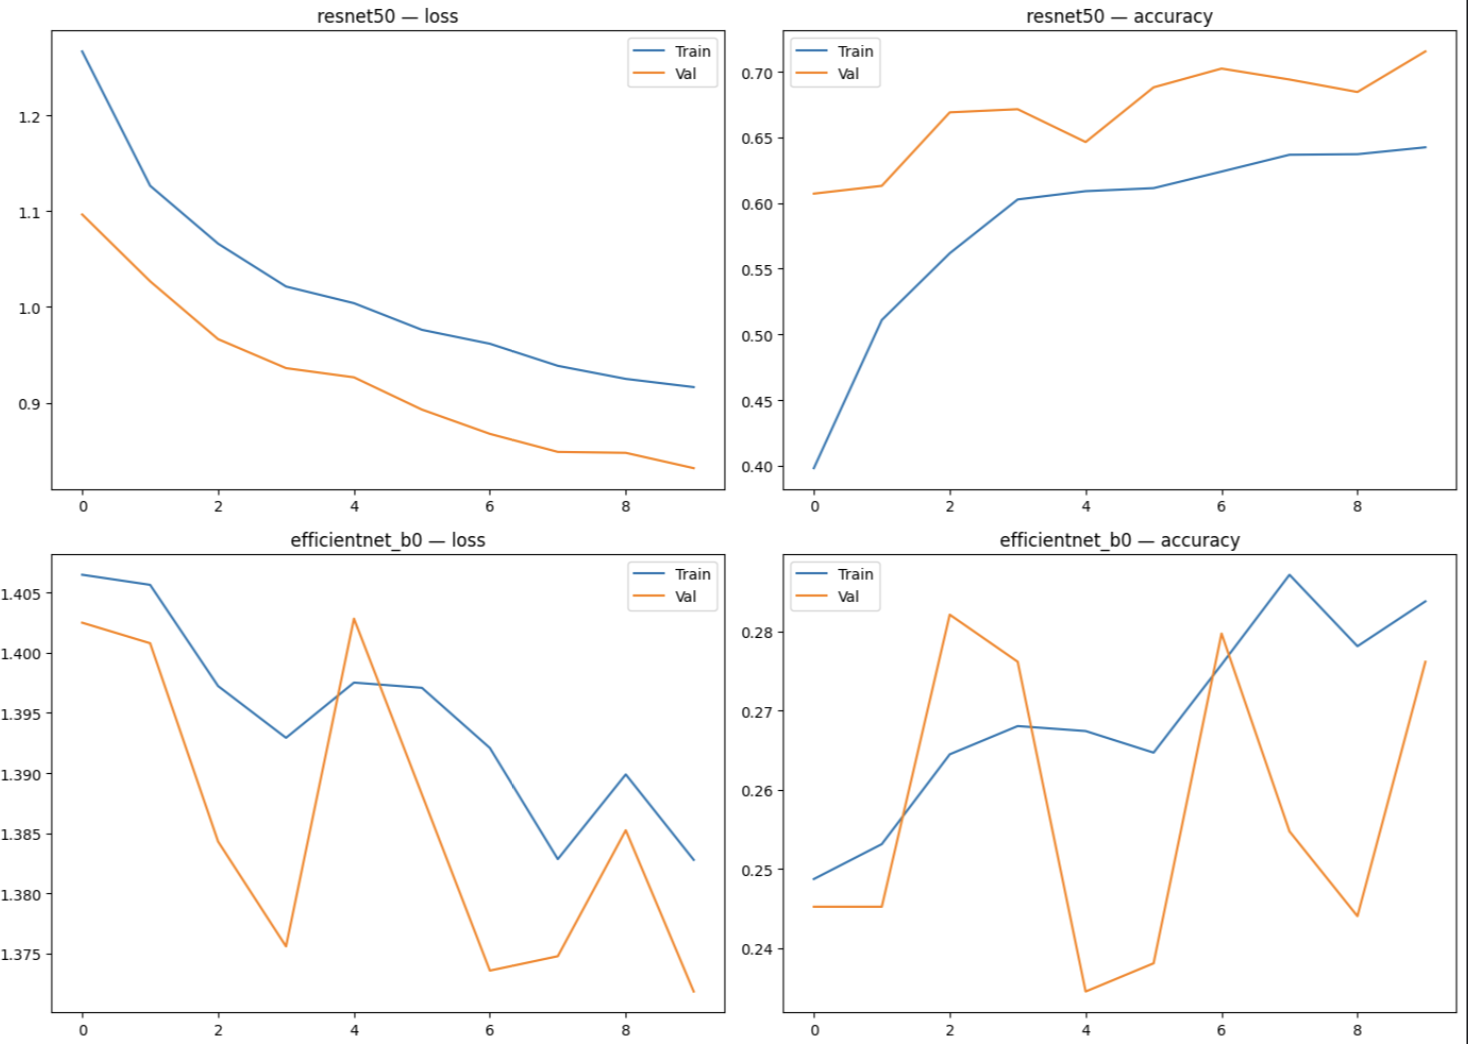
\includegraphics[width=\textwidth]{figure2tf.png}
\caption{TensorFlow training and validation loss and accuracy over 10 epochs. Top: ResNet-50. Bottom: EfficientNet-B0.}
\label{fig:tfcurves}
\end{figure}

\noindent TensorFlow ResNet-50 improves steadily (train loss 1.267 $\to$ 0.916, validation loss 1.097 $\to$ 0.832, validation accuracy 71.6\% at epoch 10), but starts from a much worse point and ends far below the PyTorch models. TensorFlow EfficientNet-B0 barely learns: its loss stays at about 1.38--1.41, which is essentially $\ln 4\approx1.386$, the loss of a model that outputs a uniform distribution over four classes. Its validation accuracy oscillates between 23\% and 28\% (chance level is 25\%).

\subsection{Test-set performance}
\begin{table}[H]
\centering
\caption{TensorFlow per-class test results (400 images per class).}
\label{tab:tfclass}
\begin{tabular}{lcccccc}
\toprule
 & \multicolumn{3}{c}{ResNet-50} & \multicolumn{3}{c}{EfficientNet-B0} \\
\cmidrule(lr){2-4}\cmidrule(lr){5-7}
Class & P & R & F1 & P & R & F1 \\
\midrule
glioma      & 0.64 & 0.40 & 0.49 & 0.27 & 0.92 & 0.41 \\
meningioma  & 0.47 & 0.56 & 0.51 & 0.00 & 0.00 & 0.00 \\
notumor     & 0.66 & 0.82 & 0.73 & 0.92 & 0.12 & 0.20 \\
pituitary   & 0.70 & 0.65 & 0.67 & 0.00 & 0.00 & 0.00 \\
\midrule
Macro avg   & 0.62 & 0.61 & 0.60 & 0.30 & 0.26 & 0.15 \\
Weighted avg & 0.62 & 0.61 & 0.60 & 0.30 & 0.26 & 0.15 \\
\midrule
\textbf{Accuracy} & \multicolumn{3}{c}{\textbf{0.6081}} & \multicolumn{3}{c}{\textbf{0.2594}} \\
\bottomrule
\end{tabular}
\end{table}

\noindent The TensorFlow EfficientNet-B0 model collapsed: it never predicts meningioma or pituitary and assigns almost every image to glioma (92\% recall, 27\% precision).

\paragraph{Likely cause of the TensorFlow gap.}
The Keras pipeline feeds images scaled to $[0,1]$ into the pretrained backbones. The Keras application models expect their own input convention instead: \texttt{ResNet50} expects \texttt{resnet.preprocess\_input} (RGB$\to$BGR and ImageNet mean subtraction on $0$--$255$ pixels), and \texttt{EfficientNetB0} contains its own rescaling and expects raw $0$--$255$ pixels. With $[0,1]$ inputs the pretrained features are fed values far outside the range they were trained on, which is consistent with the near-chance behaviour of EfficientNet-B0. The PyTorch pipeline, in contrast, uses the exact ImageNet normalisation the torchvision weights expect. We therefore regard the TensorFlow numbers as reflecting a preprocessing mismatch in our pipeline, \emph{not} an inherent weakness of TensorFlow. \todo{re-run the TensorFlow notebook with the correct per-model preprocess\_input, then replace Tables~\ref{tab:summary} and~\ref{tab:tfclass}, Figure~\ref{fig:tfcurves}, Figure~\ref{fig:tfcam} and the TensorFlow discussion in Sections~\ref{sec:fwcomp} and~\ref{sec:archcomp}; if the gap closes, rewrite this paragraph as the lesson learned}

% ------------------------------------------------------------
\section{Model Interpretability: Grad-CAM}\label{sec:cam}
We applied Grad-CAM to both frameworks on the first test image (a glioma). In PyTorch we used the \texttt{pytorch-grad-cam} library on the last convolutional block; in TensorFlow we implemented Grad-CAM manually with \texttt{tf.GradientTape} on the last convolutional feature map. The heatmap is the ReLU of the gradient-weighted sum of the feature maps, upsampled to $224\times224$ and overlaid on the image (red = strongest influence).

\begin{figure}[H]
\centering
\begin{subfigure}[t]{0.49\textwidth}
  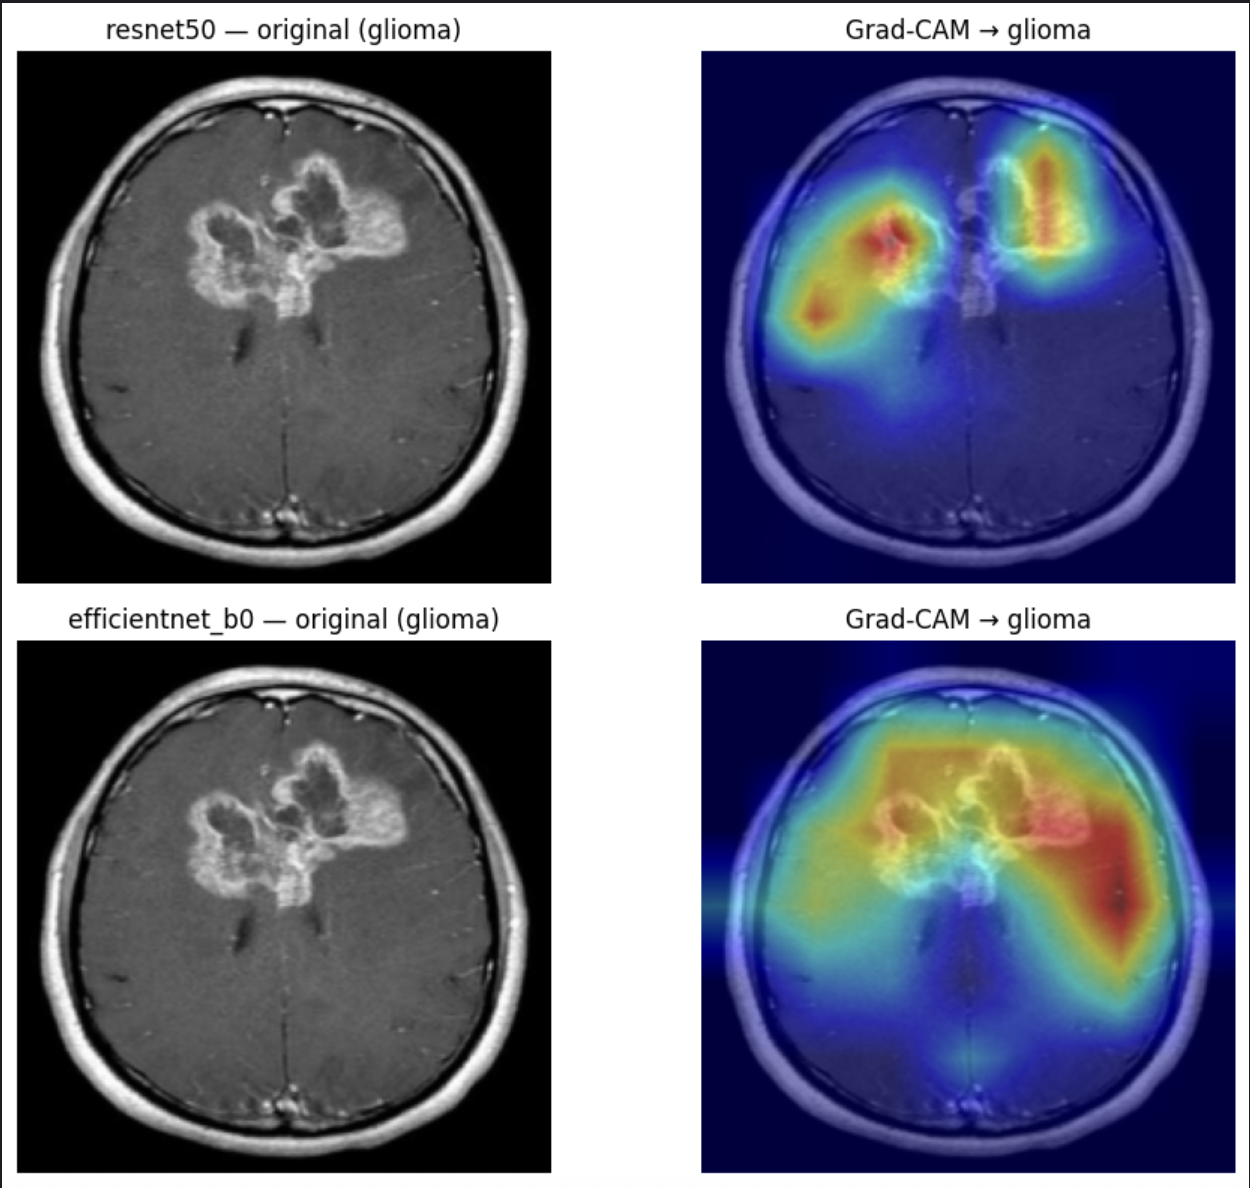
\includegraphics[width=\textwidth]{figure3pytorch.png}
  \caption{PyTorch (top: ResNet-50, bottom: EfficientNet-B0).}
  \label{fig:ptcam}
\end{subfigure}\hfill
\begin{subfigure}[t]{0.49\textwidth}
  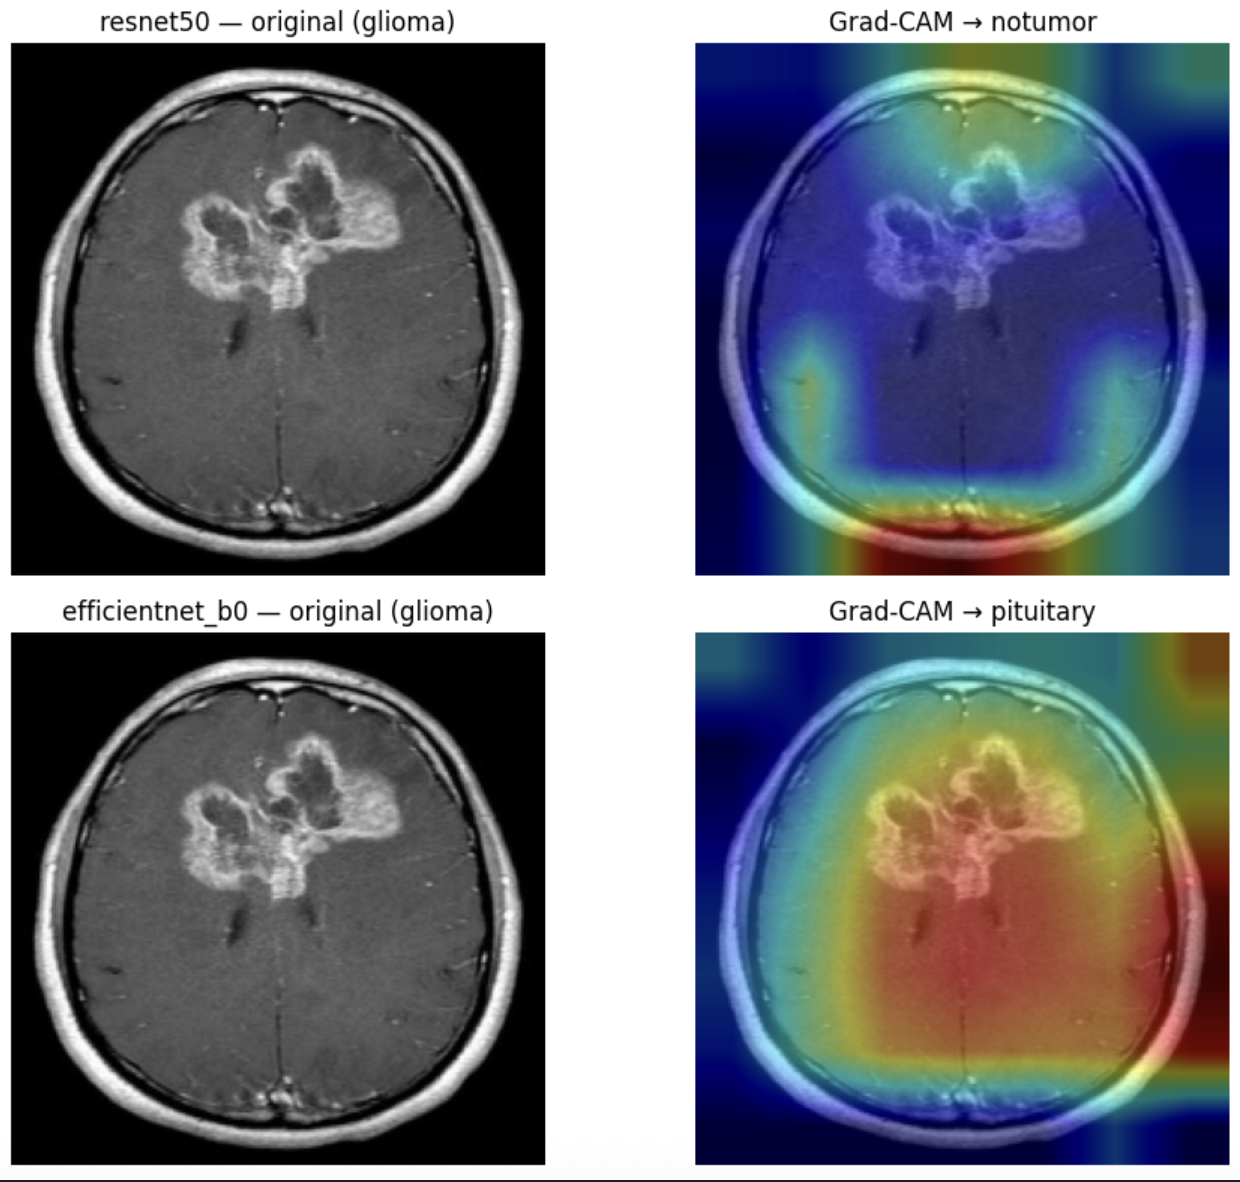
\includegraphics[width=\textwidth]{figure3tf.png}
  \caption{TensorFlow (top: ResNet-50, bottom: EfficientNet-B0).}
  \label{fig:tfcam}
\end{subfigure}
\caption{Grad-CAM for the same glioma test image. Titles show the class the heatmap was computed for.}
\label{fig:gradcam}
\end{figure}

\paragraph{Observations.}
\begin{itemize}
  \item \textbf{PyTorch ResNet-50} concentrates on the two bright, lobulated lesion regions in the frontal area and ignores the skull and background, which is the anatomically sensible behaviour.
  \item \textbf{PyTorch EfficientNet-B0} highlights the lesion but also a large part of the surrounding hemisphere; its explanation is more diffuse and less selective than ResNet-50's.
  \item \textbf{TensorFlow models} both misclassify this image (ResNet-50 predicts notumor, EfficientNet-B0 predicts pituitary), and their heatmaps are driven by the skull edge, the image border and the lower background rather than the lesion. This agrees with their low test accuracy: the features being used are not the diagnostically relevant ones.
\end{itemize}

\paragraph{Caveats.} (i)~The PyTorch heatmaps were computed for the \emph{ground-truth} class, whereas the TensorFlow heatmaps were computed for the \emph{predicted} class, so the two columns are not strictly like-for-like. (ii)~Only a single image is shown; Grad-CAM is a qualitative aid and does not prove that a model is reasoning correctly. \todo{optionally re-run Grad-CAM for both frameworks on the predicted class and on 1--2 more test images per class}

% ------------------------------------------------------------
\section{Framework Comparison: TensorFlow vs.\ PyTorch}
\label{sec:fwcomp}
\begin{table}[H]
\centering
\caption{Framework comparison on the four criteria required by the assignment.}
\label{tab:fwcomp}
\begin{tabular}{p{2.8cm}p{6.1cm}p{6.1cm}}
\toprule
\textbf{Criterion} & \textbf{PyTorch} & \textbf{TensorFlow / Keras} \\
\midrule
Ease of implementation and debugging &
Explicit training and evaluation loops give full control, and every intermediate tensor can be inspected, but we must write the loop, metrics and checkpoint logic ourselves. Pretrained models are one call away (\texttt{torchvision}). Grad-CAM was a few lines using an external library. &
\texttt{model.fit}, built-in metrics and \texttt{tf.data} pipelines make the standard workflow shorter. Debugging was harder in our case: the preprocessing mismatch caused \emph{no error}, only poor accuracy, and Keras~3 emitted input-structure warnings during Grad-CAM. Grad-CAM had to be written by hand with \texttt{GradientTape}. \\
\addlinespace
Training speed and resource utilisation &
\todo{PyTorch wall-clock time per epoch and total, and GPU memory; the notebook did not record timing} &
Measured from the training logs on a CUDA GPU: ResNet-50 about 20--21\,s per epoch after a 40\,s first epoch (about 3.7\,min for 10 epochs); EfficientNet-B0 about 18\,s per epoch after an 80\,s first epoch (about 4.0\,min). The first epoch is dominated by graph tracing and kernel autotuning; the logs also show repeated CUDA autotuning timer warnings. \\
\addlinespace
Flexibility in architecture design &
Models are ordinary Python objects: layers can be replaced in place (\texttt{model.fc = \dots}), custom forward passes and hooks are straightforward, and freezing is per-parameter. Very flexible, but also more manual. &
The functional API makes building a new head on a pretrained backbone concise, and freezing is a single flag. Reaching into a nested backbone for Grad-CAM (layer names, Keras~3 model structure) was less convenient. Flexible for standard designs, more rigid for unusual ones. \\
\addlinespace
Final performance and stability &
ResNet-50 0.8406 and EfficientNet-B0 0.8369 accuracy; smooth, monotonic loss curves for EfficientNet-B0 (the one with a saved history). &
ResNet-50 0.6081 and EfficientNet-B0 0.2594 accuracy; EfficientNet-B0 did not learn and its validation curve oscillates. As explained in Section~\ref{sec:tf}, this is most likely a preprocessing problem in our pipeline. \\
\bottomrule
\end{tabular}
\end{table}

\paragraph{A subtle difference between the two training setups.}
In PyTorch, setting \texttt{requires\_grad=False} freezes the backbone \emph{weights}, but the notebook calls \texttt{model.train()}, which keeps BatchNorm layers in training mode, so the backbone's BatchNorm running statistics are still updated on MRI data. In Keras, \texttt{base.trainable=False} also puts BatchNorm layers in inference mode, so the ImageNet statistics stay fixed. This partial domain adaptation in the PyTorch setup is a plausible additional contributor to its better results on greyscale MRI, and it shows that ``frozen backbone'' does not mean exactly the same thing in the two frameworks.

\paragraph{Conclusion.}
On ease of getting a standard model trained, Keras is faster to write; on transparency, control and debuggability, PyTorch was easier to reason about. Performance comparisons from this experiment should be read with care: the two pipelines differ in normalisation, rotation range and BatchNorm behaviour (Section~\ref{sec:preproc} and above), so the accuracy gap is confounded by these differences rather than being a clean measurement of the frameworks themselves.

% ------------------------------------------------------------
\section{Architecture, Hyperparameter and Training-Strategy Comparison}
\label{sec:archcomp}
We compared two architectures, ResNet-50 and EfficientNet-B0, under the same training strategy (frozen backbone, Adam, $10^{-3}$, batch 32, 10 epochs).

\begin{table}[H]
\centering
\caption{Architecture comparison (parameter counts are those of the backbone without classification head).}
\label{tab:archcomp}
\begin{tabular}{lcccc}
\toprule
 & \multicolumn{2}{c}{PyTorch} & \multicolumn{2}{c}{TensorFlow} \\
\cmidrule(lr){2-3}\cmidrule(lr){4-5}
 & ResNet-50 & EffNet-B0 & ResNet-50 & EffNet-B0 \\
\midrule
Backbone parameters & $\approx$23.5\,M & $\approx$4.0\,M & $\approx$23.5\,M & $\approx$4.0\,M \\
Trainable parameters & 8{,}196 & 5{,}124 & 8{,}196 & 5{,}124 \\
Test accuracy & 0.8406 & 0.8369 & 0.6081 & 0.2594 \\
Weighted F1 & 0.8368 & 0.8320 & 0.6019 & 0.1541 \\
Final val.\ accuracy & n/a & 0.9012 & 0.7155 & 0.2762 \\
\bottomrule
\end{tabular}
\end{table}

\begin{itemize}
  \item \textbf{In PyTorch the two architectures are effectively tied.} ResNet-50 is ahead by 0.37 percentage points, i.e.\ 6 of 1{,}600 test images, which is within what a different random seed could change. EfficientNet-B0 reaches this accuracy with roughly one sixth of the backbone parameters, so it is much cheaper to store and run.
  \item \textbf{In TensorFlow the architectures differ strongly}, but this reflects how each responds to the input-scaling mismatch (Section~\ref{sec:tf}) more than any intrinsic quality of the architectures.
  \item \textbf{Hyperparameters and training strategy were not varied.} We used a single setting for every model, so we cannot make claims about learning rate, batch size or optimiser sensitivity. The most informative next experiment is to unfreeze the last backbone stage(s) with a smaller learning rate (e.g.\ $10^{-4}$ to $10^{-5}$), train for more epochs with early stopping, and compare against the frozen-backbone baseline reported here. \todo{if time permits, run this experiment and add its results as a third row of the comparison}
\end{itemize}

% ------------------------------------------------------------
\section{Limitations}
\begin{itemize}
  \item \textbf{No true fine-tuning.} The backbones were fully frozen and only the head was trained for 10 epochs, which limits accuracy (84\% is well below the accuracies usually reported for fine-tuned models on this dataset).
  \item \textbf{Framework comparison is confounded.} Normalisation, rotation range and BatchNorm behaviour differ between the pipelines (Sections~\ref{sec:preproc}, \ref{sec:tf} and \ref{sec:fwcomp}), and the TensorFlow models likely suffer from a preprocessing mismatch.
  \item \textbf{Model selection on the test set.} The deployed architecture was chosen by comparing test accuracy, so the reported test accuracy of the selected model is slightly optimistic. A cleaner protocol would select on the validation set.
  \item \textbf{Single run, no variance estimate.} Each model was trained once with one seed; differences of a few tenths of a percent (such as ResNet-50 vs.\ EfficientNet-B0 in PyTorch) are not statistically meaningful.
  \item \textbf{Validation vs.\ test gap.} Validation accuracy (e.g.\ 90.1\% for PyTorch EfficientNet-B0) is noticeably higher than test accuracy (83.7\%), and similarly in TensorFlow. The validation images are a random subset of the training folder, and the dataset provides no patient identifiers, so we cannot rule out that slices from the same patient appear in both train and validation, or that the \texttt{Testing} folder has a different distribution (scanner, protocol). Validation accuracy should be treated as optimistic.
  \item \textbf{Clinically important error pattern.} Low glioma recall and over-prediction of ``notumor'' mean that many tumours would be missed. The model is not suitable for clinical use.
  \item \textbf{Metrics reporting.} Precision, recall and F1 are weighted averages (the test set is balanced, so weighted and macro averages coincide up to rounding).
  \item \textbf{Interpretability evidence is anecdotal.} Grad-CAM was shown for one image only, and the PyTorch and TensorFlow maps target different classes (Section~\ref{sec:cam}).
  \item \textbf{2D slices from one public dataset.} No 3D context, no external validation set, and no domain-shift testing.
\end{itemize}

% ------------------------------------------------------------
\section{Deployed Model and Why We Chose It}
We deploy the \textbf{PyTorch ResNet-50} model (\texttt{model/model\_\TeamID.pt}) through FastAPI.

\paragraph{Reasons.}
\begin{itemize}
  \item \textbf{Accuracy:} it has the highest test accuracy (0.8406), weighted F1 (0.8368) and precision/recall among all four models, and is far ahead of both TensorFlow models.
  \item \textbf{Consistency with training:} the PyTorch preprocessing (resize to $224\times224$, ImageNet mean/std) is simple to reproduce exactly at inference time, which the assignment requires.
  \item \textbf{Ease of serving:} the model is a single \texttt{.pt} file, loaded once at start-up with \texttt{torch.load(..., map\_location=torch.device("cpu"))}, and runs on CPU without any external service.
\end{itemize}

\paragraph{Trade-off.}
EfficientNet-B0 has about five times fewer parameters ($\approx$5.3\,M vs.\ $\approx$25.6\,M, i.e.\ roughly 20\,MB vs.\ 100\,MB in float32) and is likely faster on CPU, with an accuracy only 0.37 points lower. We nevertheless chose ResNet-50 because accuracy was our primary criterion and the CPU latency of ResNet-50 is still low enough for single-image requests. \todo{insert measured CPU latency\_ms and model file size (MB) for ResNet-50 and, if available, EfficientNet-B0 to back this choice}

\paragraph{Service configuration (\texttt{app/config.py}).}
\begin{lstlisting}[language=Python]
FRAMEWORK = "pytorch"  # Options: "pytorch" or "tensorflow"
MODEL_PATH = "model/model_T08.pt"
CLASS_NAMES = ["glioma", "meningioma", "notumor", "pituitary"]
IMAGE_SIZE = 224
\end{lstlisting}

\paragraph{Implementation of \texttt{app/main.py}.}
The service is a FastAPI application that follows the program requirements of the assignment:
\begin{itemize}
  \item \textbf{Input validation:} \texttt{POST /predict} accepts one form file named \texttt{file}. A file whose content type does not start with \texttt{image/}, or which Pillow cannot decode, is rejected with HTTP 400 and an explanatory message. Accepted images are converted to RGB.
  \item \textbf{Model loaded once:} the model is loaded in a FastAPI start-up event handler, stored in a module-level variable and put in \texttt{eval()} mode; it is never loaded inside a request.
  \item \textbf{Same preprocessing as training:} \texttt{Resize((224,224))}, \texttt{ToTensor()} and \texttt{Normalize} with the ImageNet mean/std, identical to the evaluation transform used in the PyTorch notebook.
  \item \textbf{Inference:} the forward pass runs under \texttt{torch.no\_grad()}, followed by a softmax. The predicted label is the arg-max class, \texttt{confidence} is its probability, and all probabilities are rounded to two decimals, in the class order of \texttt{CLASS\_NAMES}.
  \item \textbf{Latency:} \texttt{latency\_ms} is the wall-clock time in whole milliseconds from reading the uploaded file until the softmax output is available, so it includes decoding, preprocessing and the forward pass.
  \item \textbf{CPU and offline:} the model is mapped to CPU and the service calls no external API; it depends only on FastAPI, Uvicorn, \texttt{python-multipart}, PyTorch, torchvision, Pillow and NumPy.
  \item \textbf{Start-up and docs:} the service starts with \texttt{uvicorn app.main:app --port 8000} from inside the \texttt{\TeamID} folder, and the interactive documentation is available at \texttt{/docs}.
\end{itemize}

% ------------------------------------------------------------
\section{Example API Requests and Responses}
Both examples call \texttt{POST /predict} with an image sent as \texttt{multipart/form-data} (field name \texttt{file}). \texttt{GET /health} returns \texttt{\{"status": "ok", "framework": "pytorch", "classes": ["glioma", "meningioma", "notumor", "pituitary"]\}}. Non-image uploads receive HTTP 400.

\paragraph{Example 1: glioma MRI.}
\begin{lstlisting}[language=bash]
curl -X POST http://127.0.0.1:8000/predict -F "file=@brain_mri_001.jpg"
\end{lstlisting}
Response (status 200):
\begin{lstlisting}
TODO: paste the real JSON returned by your running service here
(framework, label, confidence, probabilities, latency_ms)
\end{lstlisting}
\todo{run the service, send a real image from data/, and paste the exact response}

\paragraph{Example 2: notumor MRI.}
\begin{lstlisting}[language=bash]
curl -X POST http://127.0.0.1:8000/predict -F "file=@brain_mri_002.jpg"
\end{lstlisting}
Response (status 200):
\begin{lstlisting}
TODO: paste the real JSON returned by your running service here
\end{lstlisting}
\todo{paste the exact response for a second image (ideally a different class)}

\end{document}